\documentclass[10pt]{beamer}

%\usepackage[backend=bibtex,firstinits=true,style=verbose-inote,citestyle=authortitle]{biblatex}
\usepackage{bm}
\usepackage{graphicx}
\usepackage{subcaption}
\usepackage{amsmath}
\usepackage{makecell}
\usepackage{filecontents}
\usepackage{biblatex}
\newcommand{\expect}[2][]{
\ifthenelse{\equal{#1}{}}{
\mathbb{E}\left[#2\right]
}{
\underset{#1}{\mathbb{E}}\left[#2\right]
}}

\newcommand{\cov}[2][]{
\ifthenelse{\equal{#1}{}}{
\text{Cov}\left[#2\right]
}{
\underset{#1}{\text{Cov}}\left[#2\right]
}}


\newcommand{\var}[2][]{
\ifthenelse{\equal{#1}{}}{
\text{Var}[#2]
}{
\underset{#1}{\text{Var}}[#2]
}}

\newcommand{\loss}[2][]{
\ifthenelse{\equal{#1}{}}{
\mathcal{L}(#2)
}{
\mathcal{L}_{#1}(#2)
}}

\newcommand{\kl}[2]{
\text{D}_\text{KL}[#1 \parallel #2]
}

\newcommand{\R}{\mathbb{R}}
%\newcommand{\Prob}{\mathbb{P}}

\newcommand{\1}[1]{\mathds{1}\{#1\}}


%\usecolortheme{dolphin}
\setbeamertemplate{navigation symbols}{}
\setbeamertemplate{section in toc}{\inserttocsectionnumber.~\inserttocsection}

\begin{filecontents*}{references.bib}
@incollection{DGR,
title = {Continual Learning with Deep Generative Replay},
author = {Shin, Hanul and Lee, Jung Kwon and Kim, Jaehong and Kim, Jiwon},
booktitle = {Advances in Neural Information Processing Systems 30},
editor = {I. Guyon and U. V. Luxburg and S. Bengio and H. Wallach and R. Fergus and S. Vishwanathan and R. Garnett},
pages = {2990--2999},
year = {2017},
publisher = {Curran Associates, Inc.},
url = {http://papers.nips.cc/paper/6892-continual-learning-with-deep-generative-replay.pdf}
}
@incollection{MeRGAN,
title = {Memory Replay GANs: Learning to Generate New Categories without Forgetting},
author = {Wu, Chenshen and Herranz, Luis and Liu, Xialei and wang, yaxing and van de Weijer, Joost and Raducanu, Bogdan},
booktitle = {Advances in Neural Information Processing Systems 31},
editor = {S. Bengio and H. Wallach and H. Larochelle and K. Grauman and N. Cesa-Bianchi and R. Garnett},
pages = {5962--5972},
year = {2018},
publisher = {Curran Associates, Inc.},
url = {http://papers.nips.cc/paper/7836-memory-replay-gans-learning-to-generate-new-categories-without-forgetting.pdf}
}
@article{DGM,
  author    = {Oleksiy Ostapenko and
               Mihai Marian Puscas and
               Tassilo Klein and
               Patrick J{\"{a}}hnichen and
               Moin Nabi},
  title     = {Learning to Remember: {A} Synaptic Plasticity Driven Framework for
               Continual Learning},
  journal   = {CoRR},
  volume    = {abs/1904.03137},
  year      = {2019},
  url       = {http://arxiv.org/abs/1904.03137},
  archivePrefix = {arXiv},
  eprint    = {1904.03137},
  timestamp = {Wed, 24 Apr 2019 12:21:25 +0200},
  biburl    = {https://dblp.org/rec/bib/journals/corr/abs-1904-03137},
  bibsource = {dblp computer science bibliography, https://dblp.org}
}
@InProceedings{HAT,
  title = 	 {Overcoming Catastrophic Forgetting with Hard Attention to the Task},
  author = 	 {Serra, Joan and Suris, Didac and Miron, Marius and Karatzoglou, Alexandros},
  booktitle = 	 {Proceedings of the 35th International Conference on Machine Learning},
  pages = 	 {4548--4557},
  year = 	 {2018},
  editor = 	 {Dy, Jennifer and Krause, Andreas},
  volume = 	 {80},
  series = 	 {Proceedings of Machine Learning Research},
  address = 	 {Stockholmsmässan, Stockholm Sweden},
  month = 	 {10--15 Jul},
  publisher = 	 {PMLR},
  pdf = 	 {http://proceedings.mlr.press/v80/serra18a/serra18a.pdf},
  url = 	 {http://proceedings.mlr.press/v80/serra18a.html},
  abstract = 	 {Catastrophic forgetting occurs when a neural network loses the information learned in a previous task after training on subsequent tasks. This problem remains a hurdle for artificial intelligence systems with sequential learning capabilities. In this paper, we propose a task-based hard attention mechanism that preserves previous tasks’ information without affecting the current task’s learning. A hard attention mask is learned concurrently to every task, through stochastic gradient descent, and previous masks are exploited to condition such learning. We show that the proposed mechanism is effective for reducing catastrophic forgetting, cutting current rates by 45 to 80. We also show that it is robust to different hyperparameter choices, and that it offers a number of monitoring capabilities. The approach features the possibility to control both the stability and compactness of the learned knowledge, which we believe makes it also attractive for online learning or network compression applications.}
}
\end{filecontents*}

\addbibresource{references.bib}


\title{Generative Memory for Continual Learning}
%\subtitle{}
\author{Ivan Skorokhodov}
%\date{}
%\logo{
\includegraphics[height=1cm]{images/ipavlov-logo.png}}

\newcommand{\citepaper}[1]{\citetitle{#1} by \citeauthor{#1}}

%\graphicspath{{./images}}

%\usetheme{lucid}
\begin{document}

\begin{frame}
    \titlepage
\end{frame}


\begin{frame}
    \frametitle{Contents}
    \tableofcontents
\end{frame}

\section{Deep Generative Replay}
\begin{frame}
    \frametitle{Deep Generative Replay (DGR) \footnote{\citepaper{DGR}, NeurIPS 2017}}
    \framesubtitle{Main idea (1/3)}
    
    \begin{itemize}
        \item Train a generator $G_1$, train a classifier $C_1$ for task \#1
        \item For task $t > 1$ generate images with $G_{t-1}$, generate labels with $C_{t-1}$ to obtain a dataset $\hat{D}_{:t}$
        \item Train on both $\hat{D}_{:t}$ and $D_t$ (real data for task $t$) jointly
        \item Note: it's not clear from the paper if they trained $C_t$ on the logits of $C_{t-1}$ or its one-hot predictions
        \item Note: it's a bit odd that they do not train conditional generator
    \end{itemize}
    
    \[
    \mathcal{L} = r \expect[(\boldsymbol{x}, \boldsymbol{y}) \sim D_{i}]{L\left(C_t(\boldsymbol{x}), \boldsymbol{y}\right)}+(1-r) \expect[\boldsymbol{x}' \sim G_{t-1}]{L(C_t(\boldsymbol{x}'), C_{t-1}(\boldsymbol{x}'))}
    \]
\end{frame}

\begin{frame}
    \frametitle{Deep Generative Replay (DGR)}
    \framesubtitle{Illustration (2/3)}

    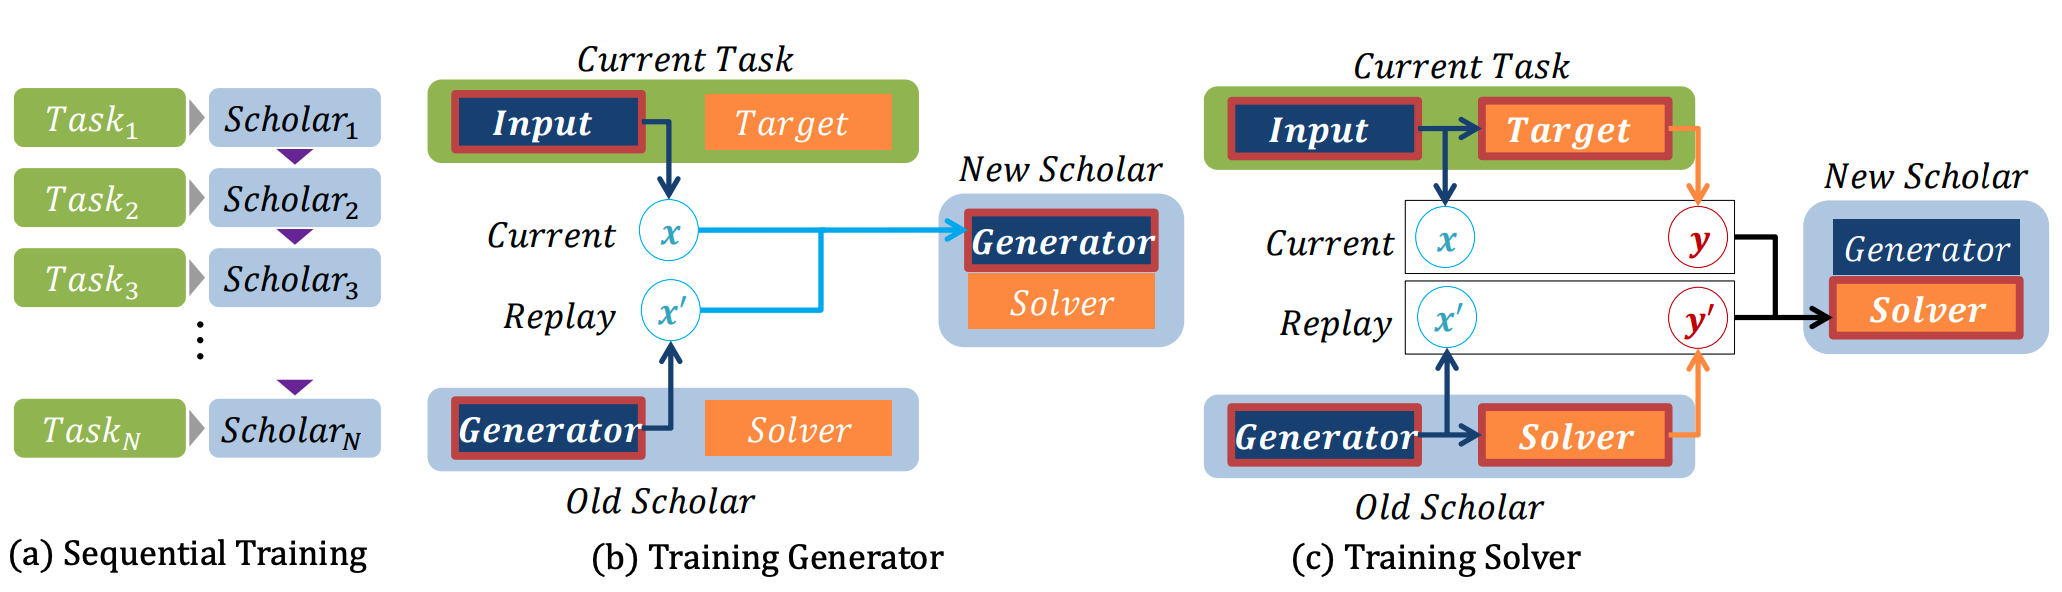
\includegraphics[width=\textwidth]{images/dgr.png}
\end{frame}

\begin{frame}
    \frametitle{Deep Generative Replay (DGR)}
    \framesubtitle{Results on permuted MNIST (3/3)}
    
    \centering
    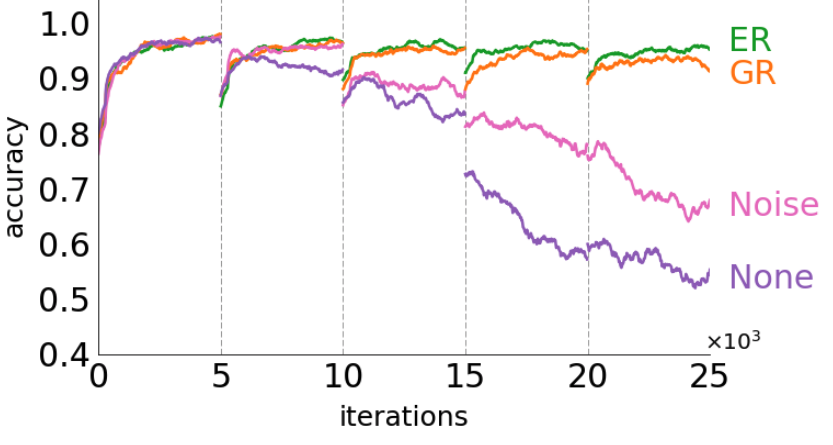
\includegraphics[width=0.5\textwidth]{images/dgr-results}
    
    \begin{itemize}
        \item 5 tasks
        \item ER --- Joint Multi-Task baseline
        \item Noise --- feeding random noise instead of images into $C_{t-1}$ to distill knowledge
    \end{itemize}
\end{frame}

%\section{CloGAN}
%They report that VAE performs worse.
\section{MeRGAN}
\begin{frame}
    \frametitle{Memory Replay GAN \footnote{\citepaper{MeRGAN}, NeurIPS 2018}}
    \framesubtitle{Main idea (1/3)}
    
    \begin{itemize}
        \item Idea is simple: train a generative memory $G_t$, save its snapshot before each new task and distill its knowledge into a new one $G_{t+1}$
        \item There are two ways to distill the knowledge
        \begin{itemize}
            \item Generate synthetic data and mix it into a new one $S'_t$ (Joint Retraining)
            \item Perform real knowledge distillation (Replay Alignment):
            \[
            \mathcal{L}_G = L_G(\theta_t, S_t) + \lambda \expect[z \sim p_z, c \sim U(0, t-1)]{\left\| G_t(z, c) - G_{t-1}(z, c) \right\|^2}
            \]
        \end{itemize}
        \item Also train a classifier on top of GAN
    \end{itemize}
\end{frame}

%\section{LAMAL}
\begin{frame}
    \frametitle{Memory Replay GAN (MeRGAN)}
    \framesubtitle{Illustration (2/3)}
    
    \centering
    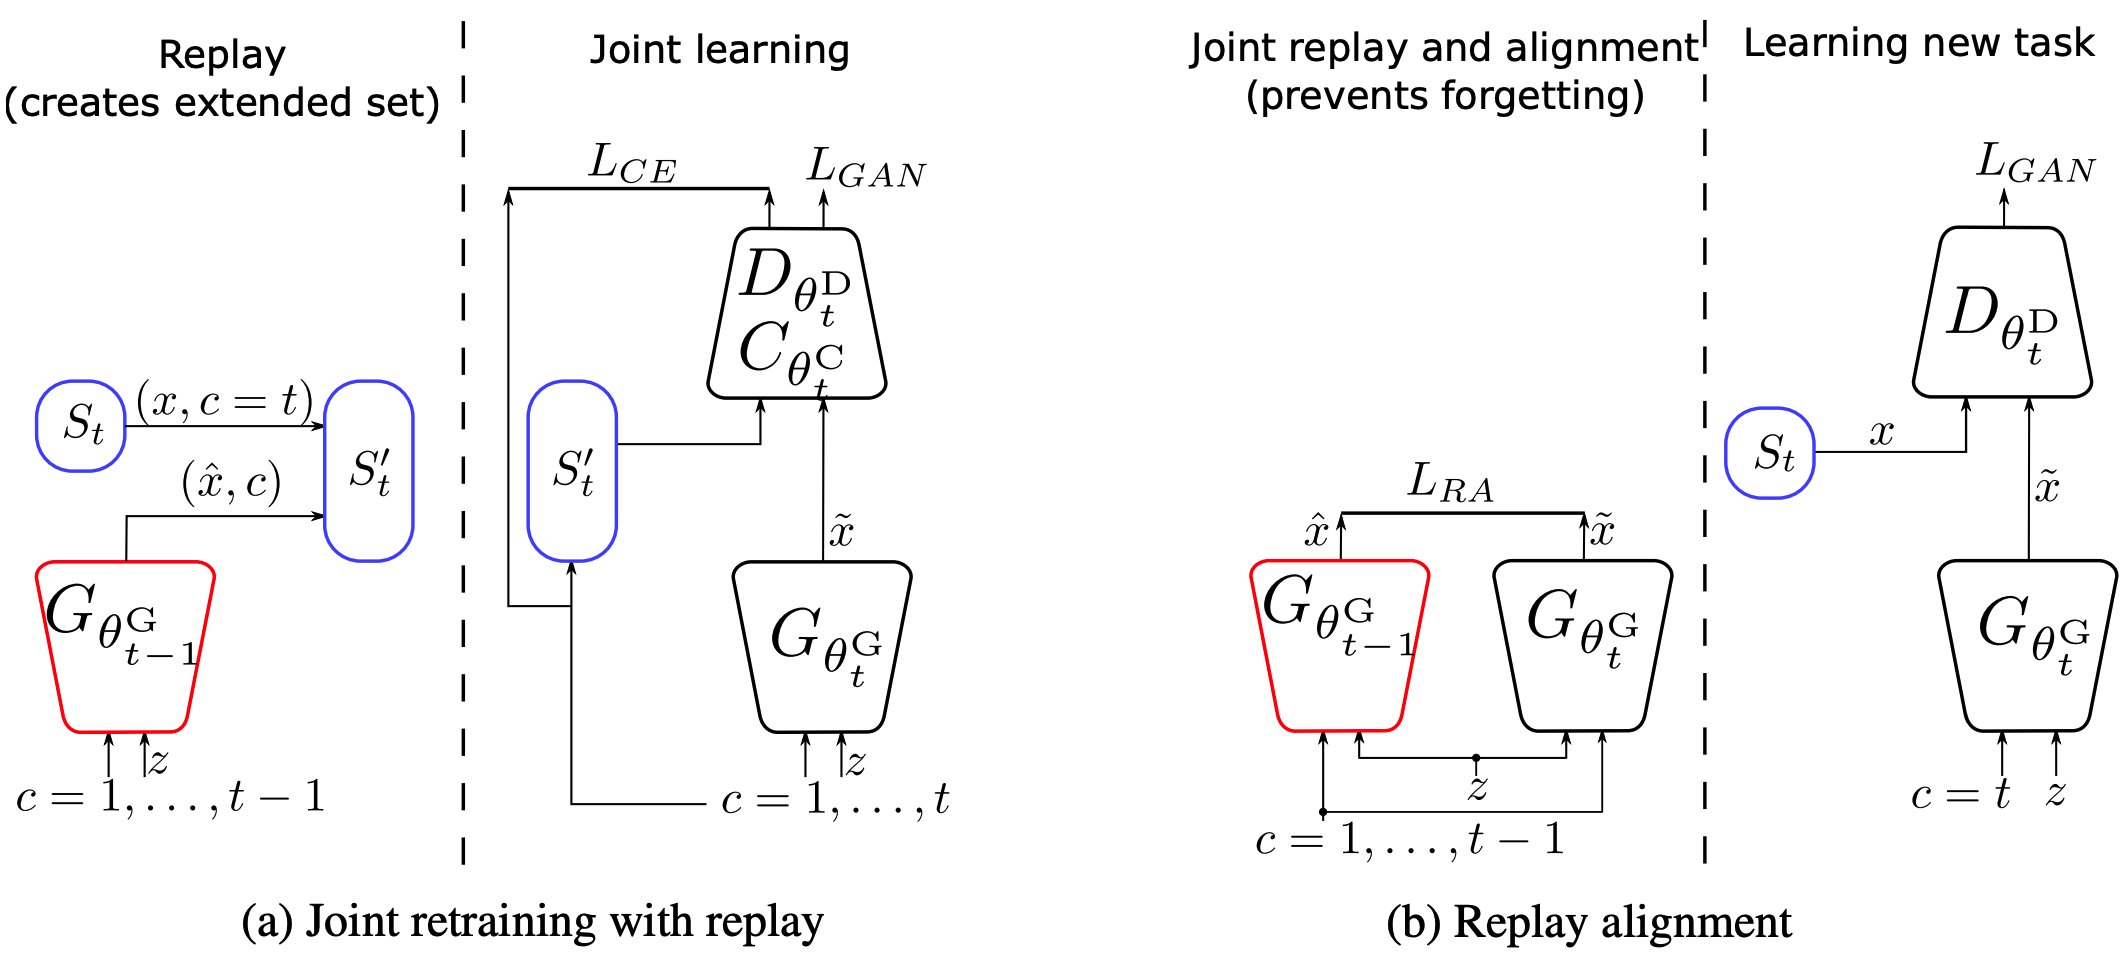
\includegraphics[width=\textwidth]{images/mergan.png}
\end{frame}

\begin{frame}
    \frametitle{Memory Replay GAN (MeRGAN)}
    \framesubtitle{Results (3/3)}
    
    \centering
    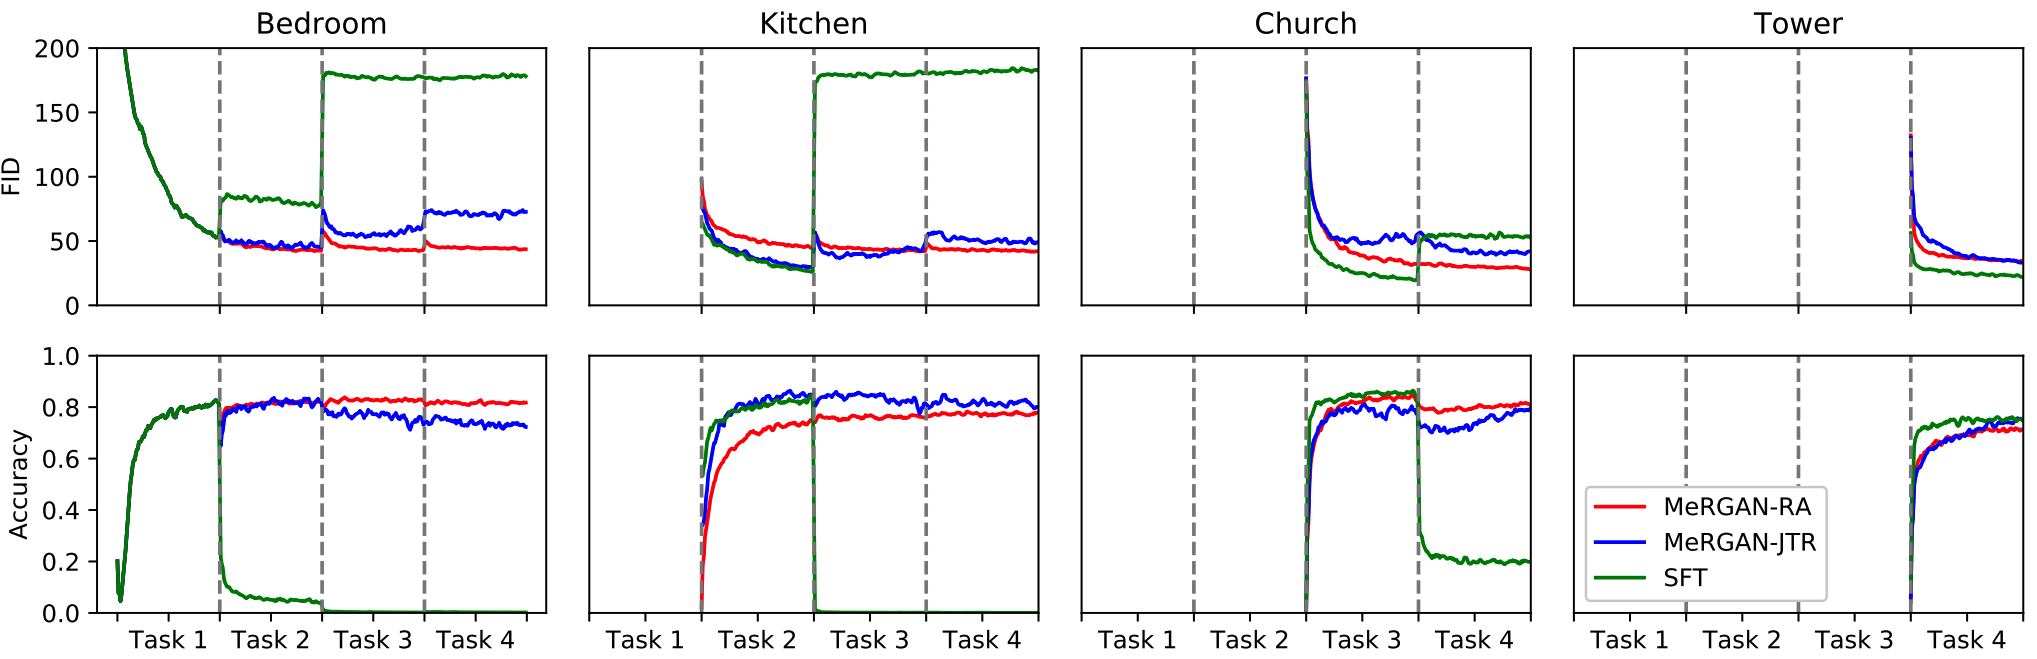
\includegraphics[width=0.8\textwidth]{images/mergan-results}
    
    \begin{itemize}
        \item SFT (sequential fine tuning) is no tricks at all
        \item Replay Alignment tends to work better
        \item Authors are not clear about how they have measured the accuracy, as far as I got --- they have trained a classifier on real data and measured its performance on the fake data.
    \end{itemize}
\end{frame}

\section{Dynamic Generative Memory}
\begin{frame}
    \frametitle{Dynamic Generative Memory (DGM) \footnote{\citepaper{DGM}, arxiv}}
    \framesubtitle{Main idea (1/3)}
    
    \begin{itemize}
        \item Authors consider class-incremental learning (just as we do): classes arrive sequentially and we evaluate the performance on all the tasks
        \item They do not run any kind of knowledge distillation and follow HAT\footnote{\citepaper{HAT}, ICML 2018} approach instead
        \item More precisely, for task $t$, for layer $l$ of the generator they train a binary mask $m_l^t$ and multiply layer's weights on this mask
        \item Binary mask $m_l^t$ is regularized to be sparse
        \item Previously learned weights are not updated in the future (but network can learn to ignore them by learning the corresponding mask)
        \item But compared to HAT, authors are cheating: they add new neurons to the generator after each task to preserve its capacity
    \end{itemize}
\end{frame}

\begin{frame}
    \frametitle{Dynamic Generative Memory (DGM)}
    \framesubtitle{Illustration (2/3)}
    
    \centering
    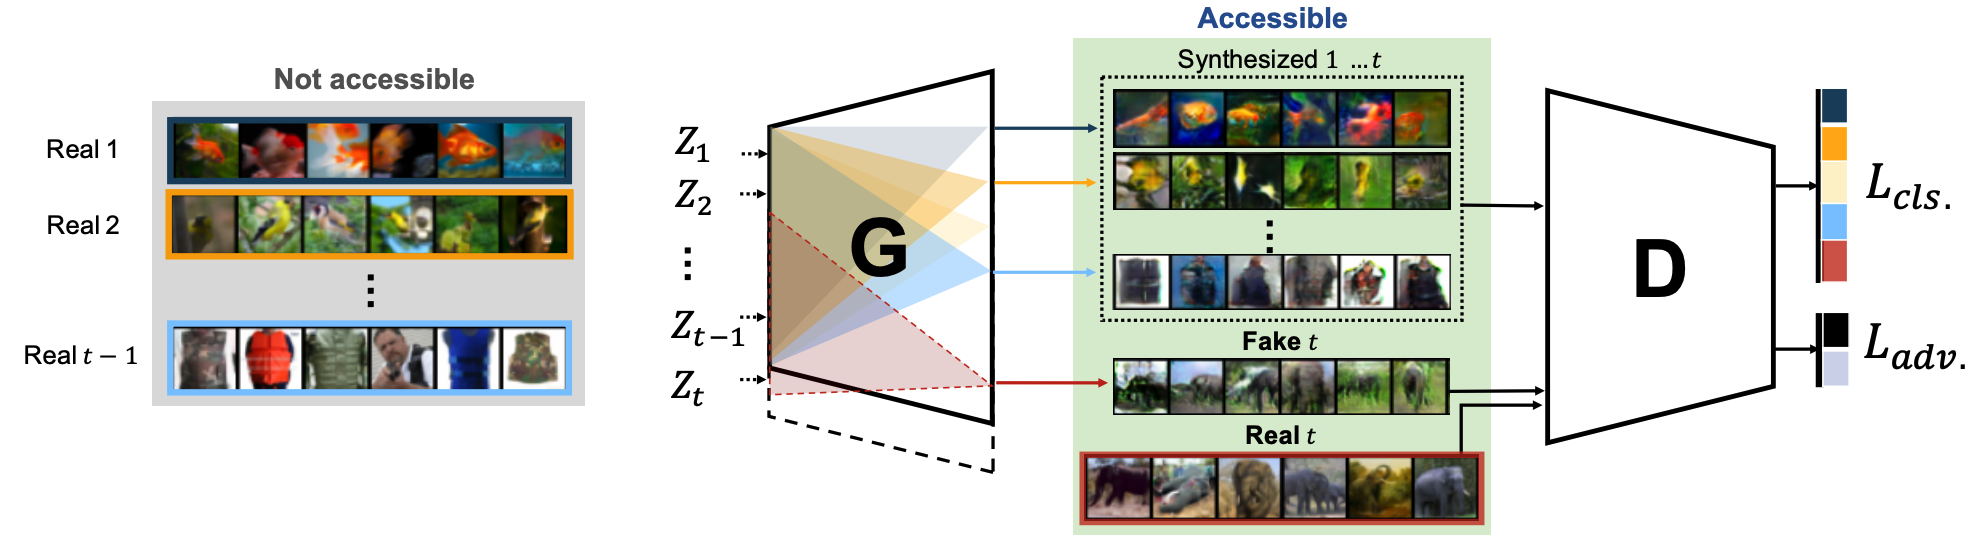
\includegraphics[width=\textwidth]{images/dgm}
\end{frame}

\begin{frame}
    \frametitle{Dynamic Generative Memory (DGM)}
    \framesubtitle{Results (3/3)}
    
    \centering
    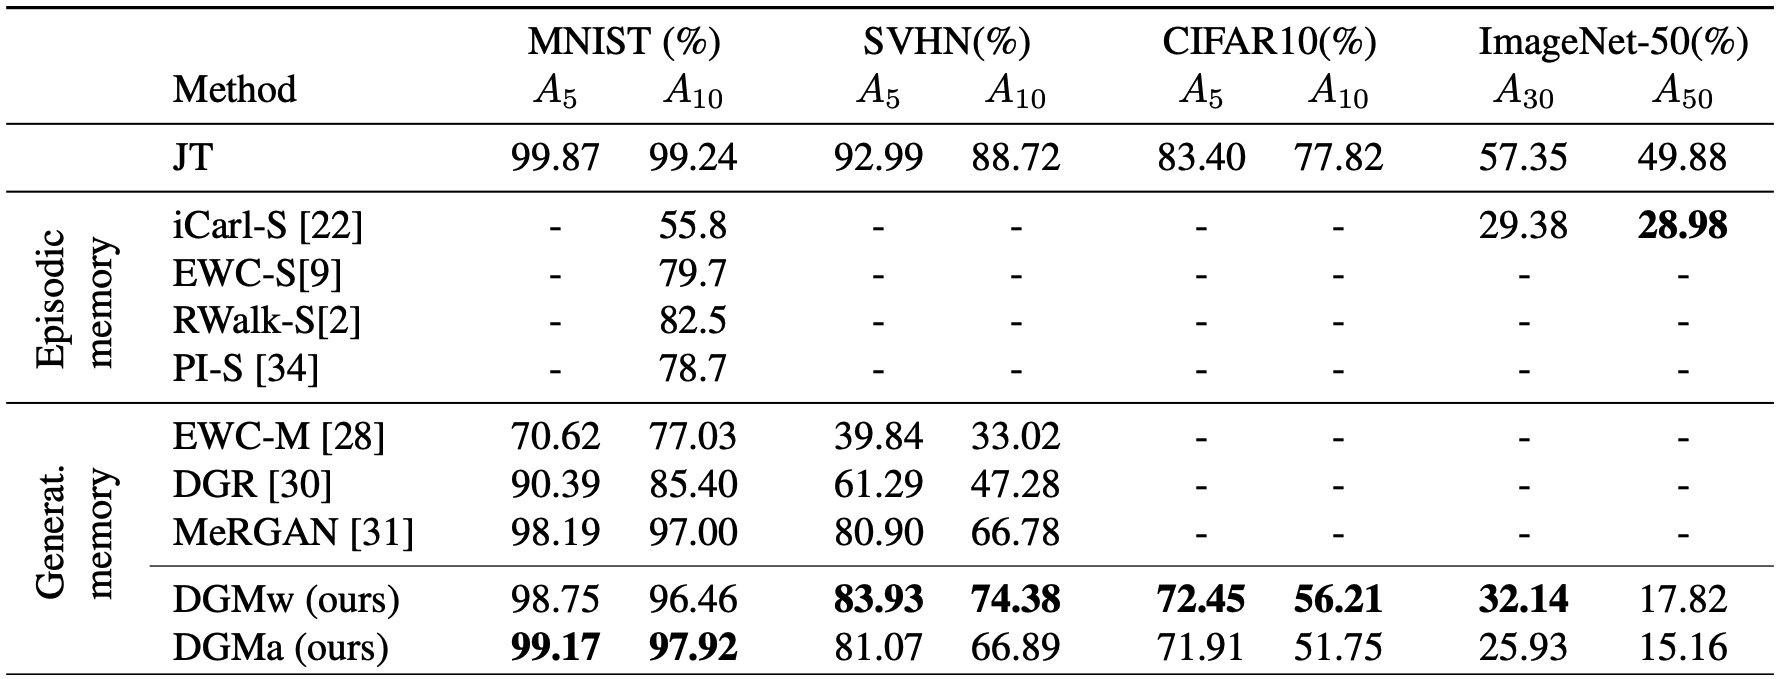
\includegraphics[width=\textwidth]{images/dgm-results}
    
    \begin{itemize}
        \item Here $A_n$ is the performance on $n$ previously seen classes
        \item For ImageNet-50 they train for 5 tasks, 10 classes per task
        \item They do not state it clearly, but as far as I got they use 5 and 10 tasks for other datasets
    \end{itemize}
\end{frame}

\section{Latent Generative Memory}
\begin{frame}
    \frametitle{Latent Generative Memory}
    \framesubtitle{Main idea (1/2)}
    
    \begin{itemize}
        \item Let's get rid of separate knowledge distillation step (it is questionable both biologically and practically)
        \item So let's train GM and Classifier jointly
        \item Since training GM in the visual space is tough, let's train it in the feature space
        \item Make the GM reside in ``deep'' layers of the Classifier and hallucinate
    \end{itemize}
\end{frame}

\begin{frame}
    \frametitle{Latent Generative Memory}
    \framesubtitle{Illustration (2/2)}

    \centering
    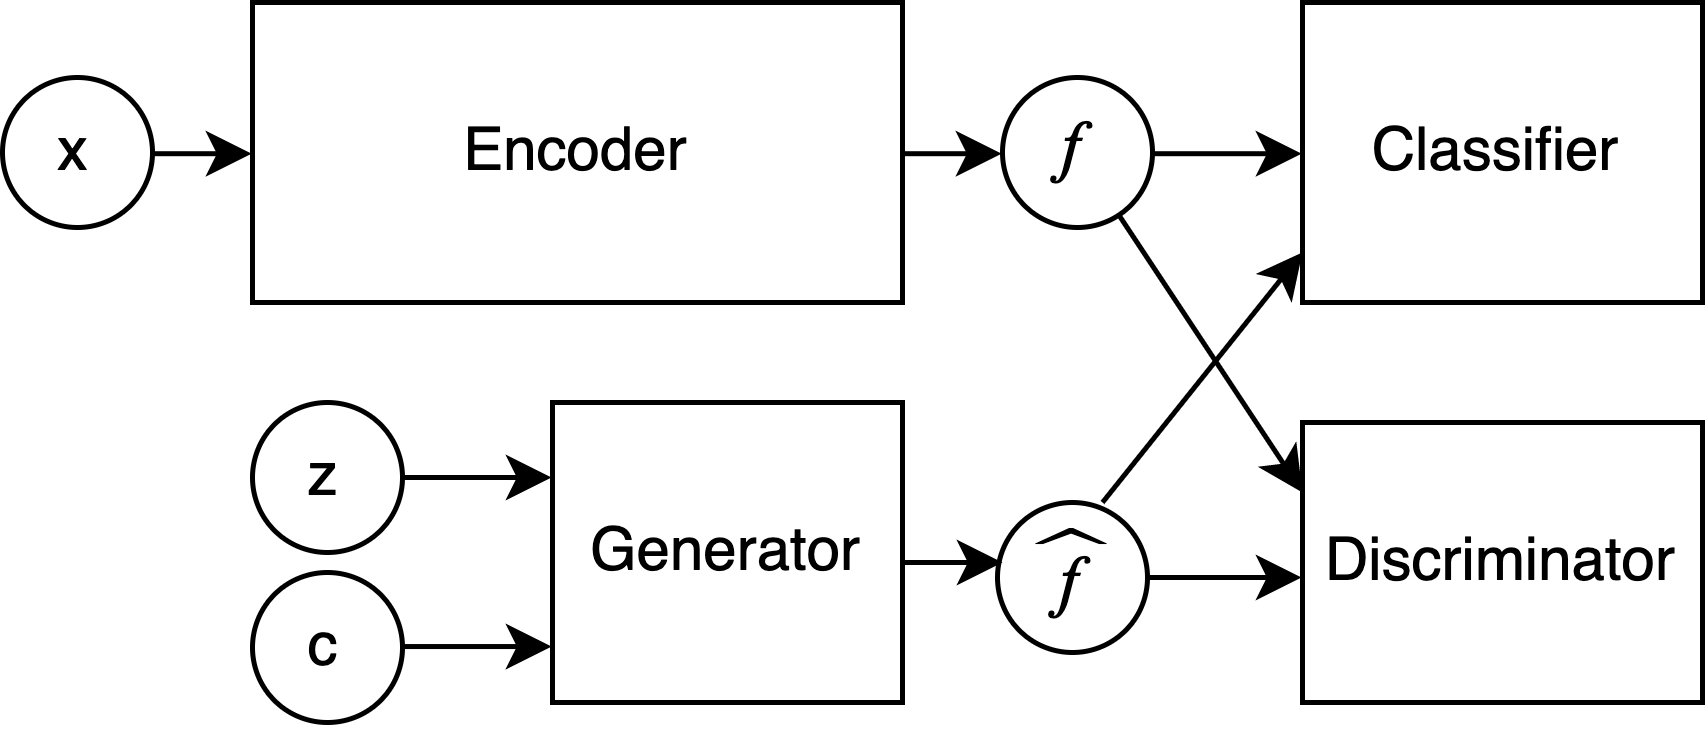
\includegraphics[width=0.5\textwidth]{images/latent-genmem}
    
    \begin{itemize}
        \item For task $t=1$ we train the model normally
        \item For task $t > 1$ generate a lot of fake memories with $G_{t-1}$ of previously seen classes
        \item Train Classifier to correctly distinguish these fake memories
        \item Question \#1: how to avoid knowledge distillation for Generator?
        \item Question \#2: what if Encoder will start changing the embedding manifold? Then our fake memories will not correspond to actual embeddings. Maybe we can introduce prototypes to resolve this?
    \end{itemize}
\end{frame}

%\begin{frame}
%    \frametitle{Prototypical Generative Memory}
%    \framesubtitle{Main idea (1/2)}
%    
%    \begin{itemize}
%        \item How can we force Encoder not to change output mapping for previous classes?
%        \item We can use prototypes and make uit
%    \end{itemize}
%\end{frame}



\end{document}
